\section{Counterfactual Prediction}

\begin{frame}{Finding a Prediction Algorithm}
    \begin{columns}
    \begin{column}{0.6\linewidth}
    Need to find a prediction algorithm to generate synthetic (counterfactual) control data post-treatment. \\
    This algorithm must be:
      \begin{enumerate}
         \item {Excellent at modeling non-linear relationships}
         \item {Robust to unobserved heterogeneity across space and time}
         \item {Suitable for high-dimensional space}
      \end{enumerate}
      \vspace{5pt}
    \footnotesize{Note: Both discrete and continuous estimands are considered. The Application section elaborates.}
    \end{column}
    \begin{column}{0.4\linewidth}
      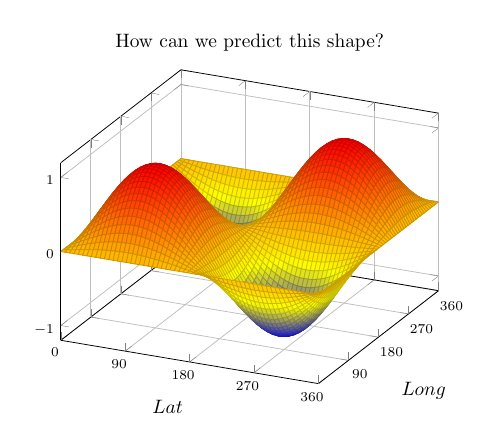
\begin{tikzpicture}[scale=0.70]
      \begin{axis} [
        title = {How can we predict this shape?},
        xtick = {0,90,...,360},
        ytick = {90,180,...,360},
        xlabel = $Lat$, ylabel = $Long$,
        ticklabel style = {font = \scriptsize},
	grid]
        \addplot3 [surf, domain=0:360, samples=60] 
        	{ sin(x)*sin(y) };
        \end{axis}
        \end{tikzpicture}
    \end{column}
  \end{columns}
\end{frame}

\begin{frame}{A Geometric Learning Approach: Graph Neural Networks}

    \begin{columns}
    \begin{column}{0.4\linewidth}
    \vspace{5pt}
      \begin{enumerate}
         \item {Invariance to Permutation, Size, and Shape: Capable of handling complex data via graph representation}
         \item {Reliable performance in non-Euclidian space: Important in high-dimensional setting}
         \item {Features and similarity: Conveys both edge and node information}
      \end{enumerate}
    \end{column}
    \begin{column}{0.6\linewidth}
      \centering
      \includegraphics[scale=0.1]{figures/gnn_summ.png}
      \caption{\footnotesize{Summary of 2-D and 3-D Graph Neural Networks}}
    \end{column}
  \end{columns}
\end{frame}

\begin{frame}{Visualizing the End Goal}

Consider treatment $Z_{it}$ occuring at $t = t^{*}$ for all locations $i$. Hypothetically, a Graph Neural Network (GNN) can predict \textcolor{cyan}{counterfactual untreated outcomes} at various locations over time:
\vspace{7pt}

  \begin{columns}
    % Split 1
    \begin{column}{0.33\linewidth}
      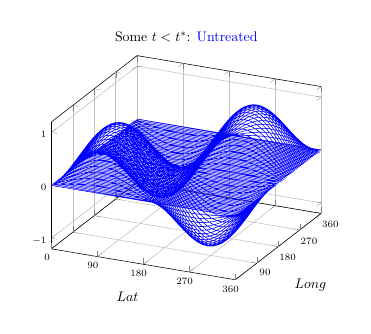
\begin{tikzpicture}[scale=0.50]
      \begin{axis} [
        title = {Some $t < t^{*}$: \textcolor{blue}{Untreated}},
        xtick = {0,90,...,360},
        ytick = {90,180,...,360},
        xlabel = $Lat$, ylabel = $Long$,
        ticklabel style = {font = \scriptsize},
	grid]
        \addplot3 [blue, domain=0:360, samples=60] 
        	{ sin(x)*sin(y) };
        \end{axis}
        \end{tikzpicture}
        \centering{\footnotesize{Pre-treatment, no treatment response, $Y_{it}(0)$}}
    \end{column}
    % Split 2
    \begin{column}{0.33\linewidth}
      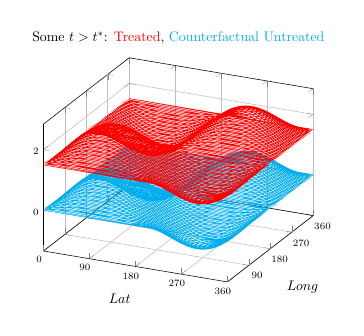
\begin{tikzpicture}[scale=0.50]
      \begin{axis} [
        title = {Some $t > t^{*}$: \textcolor{red}{Treated}, \textcolor{cyan}{Counterfactual Untreated}},
        xtick = {0,90,...,360},
        ytick = {90,180,...,360},
        xlabel = $Lat$, ylabel = $Long$,
        ticklabel style = {font = \scriptsize},
	grid]
        \addplot3 [cyan, domain=0:360, samples=60] 
        	{ sin(x)*sin(y) };
        \addplot3 [red, domain=0:360, samples=60] 
        	{ sin(x)*sin(y) + 1.5 };
        \end{axis}
        \end{tikzpicture}
        \centering{\footnotesize{Post-treatment, homogeneous response, $Y_{it}(1)$}}
    \end{column}
    % Split 3
    \begin{column}{0.33\linewidth}
      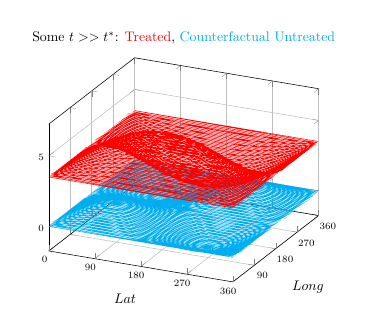
\begin{tikzpicture}[scale=0.50]
      \begin{axis} [
        title = {Some $t >> t^{*}$: \textcolor{red}{Treated}, \textcolor{cyan}{Counterfactual Untreated}},
        xtick = {0,90,...,360},
        ytick = {90,180,...,360},
        xlabel = $Lat$, ylabel = $Long$,
        ticklabel style = {font = \scriptsize},
	grid]
        \addplot3 [cyan, domain=0:360, samples=60] 
        	{ sin(x)*sin(y) };
        \addplot3 [red, domain=0:360, samples=60] 
        	{ sin(0.5*x)*3*sin(y) + 3.5 };
        \end{axis}
        \end{tikzpicture}
        \centering{\footnotesize{Post-treatment, heterogeneous response, $Y_{it}(1)$}}
    \end{column}
  \end{columns}
\end{frame}